\section{Measurement And Data Analysis}

	\subsection{Presentation Of Data}
		Since we are only interested in the peak values for our calculations and the general shape of the spectra to draw conclusions, the data is taken as photographs from the laboratory computer.
		\paragraph{Calibration}
			The calibration spectra data is presented below, the significance of the peaks and their values will be discussed in the discussion section.
		
			\begin{figure}[h]
				\caption{Data Taken During The Calibration Process}
				\centering
				\label{fig:CalibrationData}
				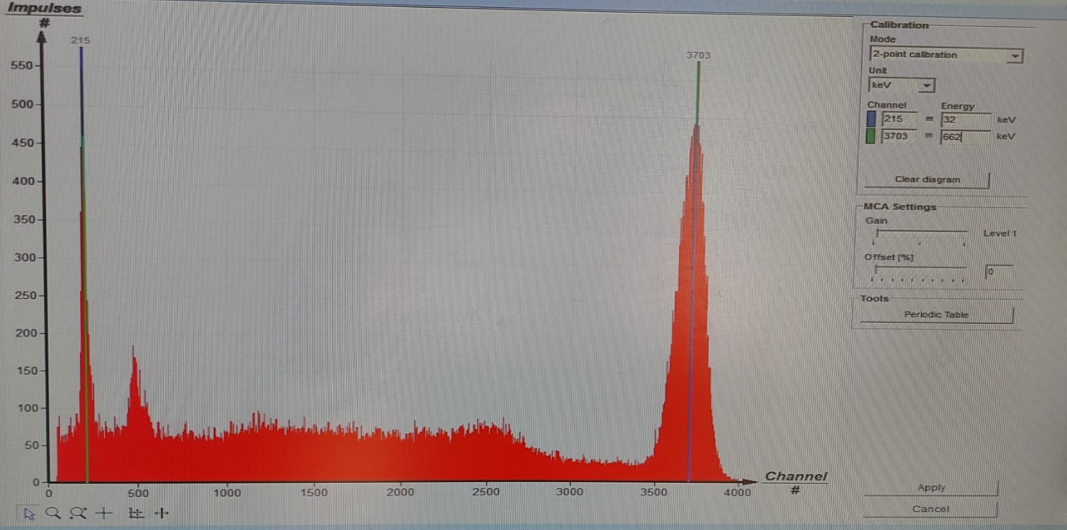
\includegraphics[width=\textwidth * 2/ 2]{images/calibration_spectra.png}
			\end{figure}
		
		\paragraph{Main}
		The raw spectra data from the experiment is presented below, this spectra was then smoothed for easier analysis. From the figure, we can see that the measurement was taken for 1331 seconds and there were 336247 total number of impulses.
		\\
		\\
		
		\begin{figure}[h!]
			\caption{Raw Data Taken During The Main Part}
			\centering
			\label{fig:RawData}
			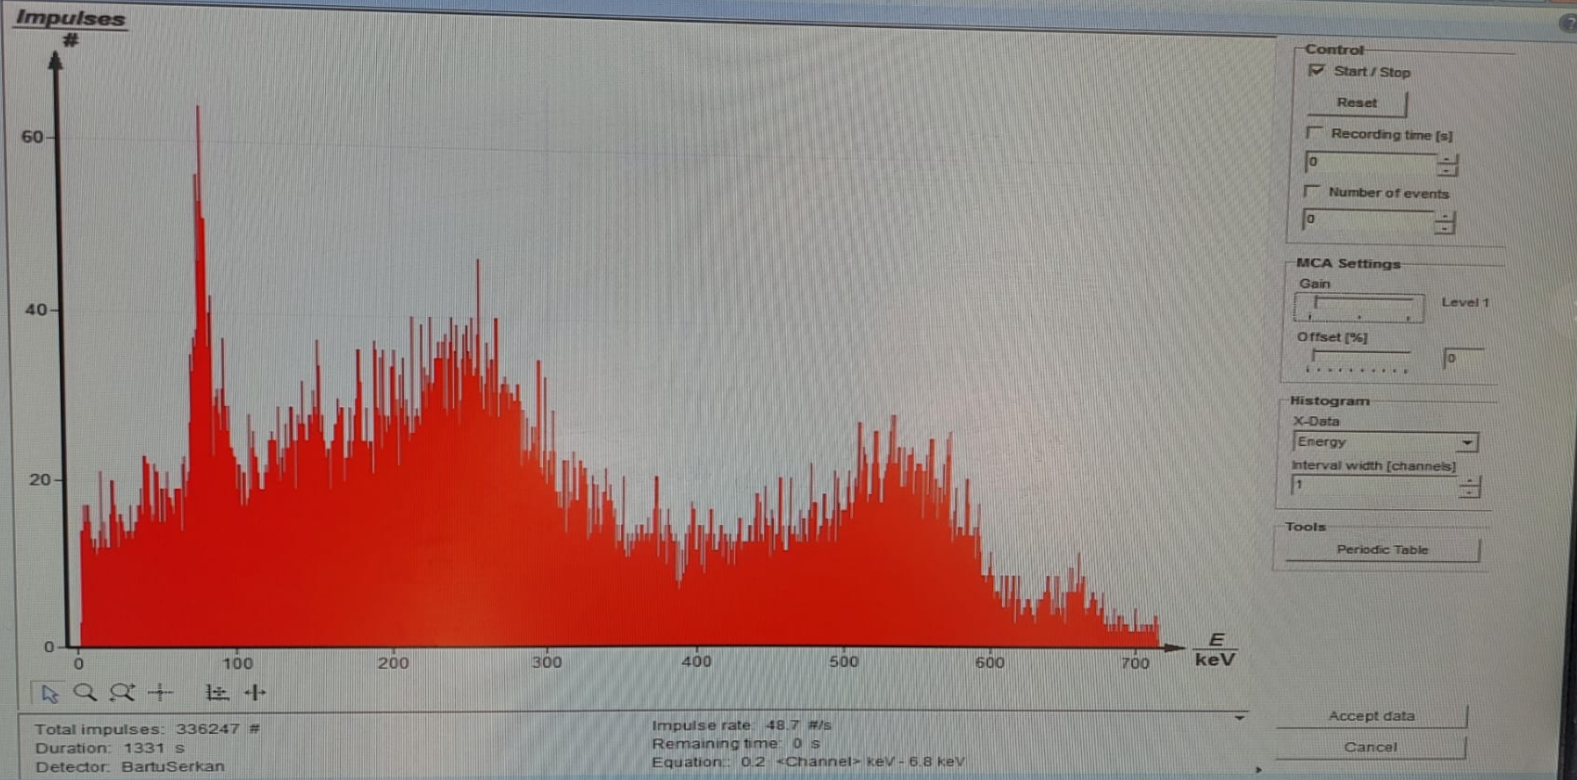
\includegraphics[width=\textwidth * 2/ 2]{images/raw_spectra.png}
		\end{figure}

	
		The smoothed spectra data from the experiment is presented below, the meanings of the three significant peaks will be discussed in the discussion section.
		\begin{figure}[h!]
			\caption{Smoothed Data Taken During The Main Part}
			\centering
			\label{fig:SmoothedData}
			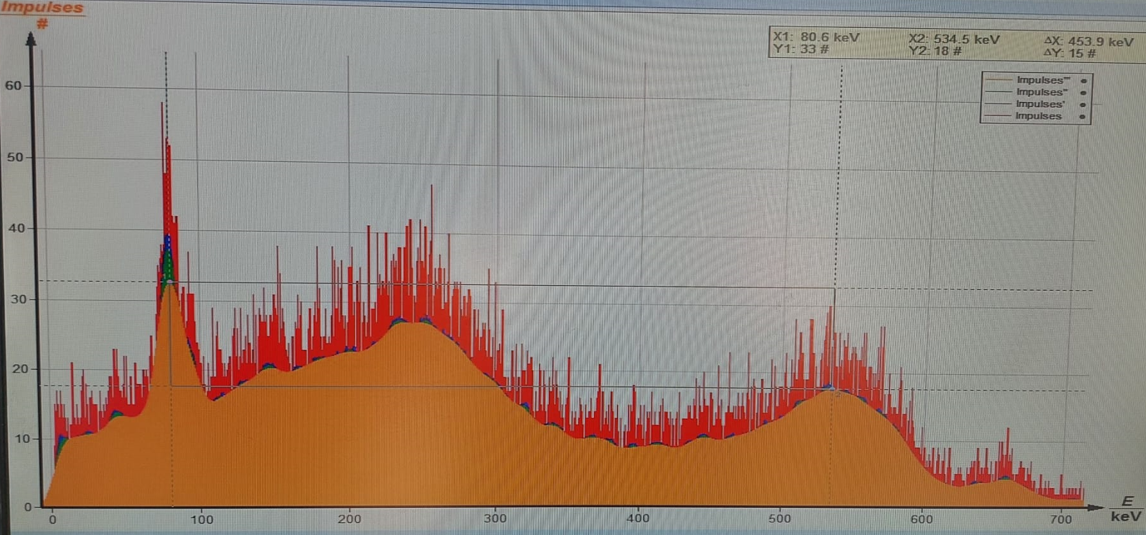
\includegraphics[width=\textwidth * 2/ 2]{images/smoothed_spectra.png}
		\end{figure}
	
	\subsection{Calculations}
		For the proof of concept, we needed to calculate the Compton wavelength which we initially knew the value of. The calculations were carried out as follows:
		\begin{align*}
			\text{incident photon wavelength, } \lambda = 1.873 * 10^{-12} m
			\\
			\text{incident photon energy, } E = 661.6 keV
			\\
			\text{scattering angle, } \phi = 30^\circ
			\\
			\text{rest mass of electron, } m_0 = 0.510998950 MeV / c^2
			\\
			\frac{1}{E'} - \frac{1}{E} = \frac{1}{m_0 c^2} (1 - cos \phi)
			\\
			E' = 563.82 keV
			\\
			E' = hc / \lambda'
			\\
			\lambda' = 0.0219928 \si{\angstrom}
			\\
			\lambda = 0.0187311 \si{\angstrom}
			\\
			\lambda_c = \frac{\lambda' - \lambda}{(1 - cos \theta)} = 0.0243457 \si{\angstrom} \text{, the Compton wavelength}
			\end{align*}
			